\begin{frame}{Eulerian Model: Conservation of Mass or Continuity Equation}
    \begin{equation} \label{gc2_eqn}
\frac{1}{\rho_r{}_q}(\frac{\partial}{\partial t }(\alpha_q\rho_q) + \nabla\cdot(\alpha_q\rho_q\vec{v_q})= \sum_{p=1}^{n} (\Dot{m_p{}_q}-\Dot{m_q{}_p}))
\end{equation}
where:\\
$\alpha_q = volume \:fraction \:of \:the \:q^{th} \:phase$\\
$\rho_q = density\:of \:the\: q^{th} \:phase$\\
$\vec{v_q} = velocity\: of\: the\: q^{th}\: phase$\\
$\Dot{m_p{}_q} = mass\: transfer\: from\: phase\: p\: to\: phase\: q$\\
$\Dot{m_q{}_p} = mass\: transfer\: from\: phase\: q\: to\: phase\: p\: $\\
\end{frame}

\begin{frame}{Eulerian Model: Conservation of Mass or Continuity Equation}
    The continuity equation or the volume fraction equation will not solved for the primary phase, the primary phase volume fraction will be computed based on the following constraint:\\
    \begin{equation}
        \sum_{p=1}^{n} \alpha_q = 1
    \end{equation}
    The volume fraction equation may be solved either through \textbf{Implicit} or \textbf{Explicit} \textbf{time discretization}. \textbf{Implicit} discretization is used for \textbf{stratified flows} while \textbf{Explicit} discretization is used for \textbf{jet flows}.
\end{frame}

\begin{frame}{Explicit Scheme: Volume Fraction Discretization Scheme}
    \begin{equation}
        \frac{\alpha_q^{n+1}\rho_q^{n+1}-\alpha_q^{n}\rho_q^{n}}{\Delta t}\:V \:+\:\sum_{f}(\rho_q U_f^{n}\alpha_{q,f}^{n})=\bigg[\sum_{p=1}^{n}(\Dot{m_p{}_q}-\Dot{m_q{}_p})\bigg]\:V
    \end{equation}
where:\\
$ n\:+\:1 = index \:for \:new \:(current) \:time \:step$\\
$ n = index\:for \:previous\: time \:step$\\
$\alpha_{q,f} = face\: value\: of\: q^{th}\: volume\: fraction,\: computed\: from\: the\: first-order\:or\:second-order\: upwind,\: QUICK,\: modified\: HRIC\:, or\: CICSAM\: scheme$\\
$V = volume\: of\: the\: cell$\\
$U_{f} = volume \: flux\: through\: the\: face,\: based\: on\: normal\: velocity\: $\\
\end{frame}

\begin{frame}{Eulerian Model: Conservation of Momentum}
    \begin{equation} \label{ffmansys_eqn}
    \begin{split}
    \frac{\partial}{\partial t }(\alpha_q\rho_q\vec{v_q}) 
    + \nabla\cdot(\alpha_q\rho_q\vec{v_q}\vec{v_q})
    = & -\alpha_q\nabla p + \nabla\cdot\Bar{\Bar{\tau_q}} 
    + \alpha_q\rho_q\vec{g} \\
    &+ \sum_{p=1}^{n} (K_p{}_q(\vec{v_p}-\vec{v_q}) + \Dot{m_p{}_q}\vec{v_p{}_q} - \Dot{m_q{}_p}\vec{v_q{}_p}) 
    \end{split}
\end{equation}
where:\\
$ \Bar{\Bar{\tau_q}}\: = stress-strain \:tensor \:of \:the \:q^{th} \:phase$\\
$ \vec{g} = acceleration\:due \:to\:gravity$\\
$K_p{}_q = mean\: interphase\: momentum\: exchange\: coefficient$\\
$\Dot{m_p{}_q} = interfacial\: mass\: transfer\: between\: p^{th}\: and\:q^{th}\:phase$\\
$\vec{v_p{}_q} = relative \: velocity\: of\: the\: p^{th}\: phase\: to\: the\: q^{th}\: phase $\\
$\vec{v_q{}_p} = relative \: velocity\: of\: the\: q^{th}\: phase\: to\: the\: p^{th}\: phase $\\
\end{frame}

\begin{frame}{Eulerian Model: Conservation of Energy}
    \begin{equation}\label{gcoe_eqn}
    \begin{split}
       \frac{\partial}{\partial t }(\alpha_q\rho_q h_q)
       &+ \nabla\cdot(\alpha_q\rho_q\vec{\mu_q} h_q)=\alpha_q\frac{\partial P_q}{\partial t}+\Bar{\Bar{\tau_q}}:\nabla\vec{\mu_q}-\nabla\cdot\vec{q_q}+ ... \\ &...+S_q+\sum_{p=1}^{n}(Q_p{}_q + \Dot{m_p{}_q} h_p{}_q - \Dot{m_q{}_p} h_q{}_p)
    \end{split}
\end{equation}
where:\\
$h_q = specific\: enthalpy\: of\: the\: q^{th}\:phase,\vec{q_q} = heat \: flux $\\
$S_q = source\: term\:that \: includes\:sources\:of\:enthalpy\:(By\:default\:S_q=0) $\\
$Q_{pq} = interfacial\:heat\:transfer $, $h_{pq} = interphase\:enthalpy$\\
The heat exchange between phases must comply with the local balance conditions: 
$Q_{pq}=-Q_{qp}\:and\:Q_{qq}=0 $\\
\end{frame}

\begin{frame}{Interfacial Area Concentration: Particle Method}
    \begin{equation}\label{satovr_eqn}
    A_p = \frac{\pi d_g^2}{\frac{1}{6}\pi d_g^3}=\frac{6}{d_g}
   \end{equation}
   \centering Particle Model
   \begin{equation} \label{iacm_eqn}
    A_f{}_g=\alpha_g A_p = \frac{6\alpha_g}{d_g}
   \end{equation}
where:\\
$A_p = area\:of\:the\:particle$\\
$d_g = diameter\:of\:the\:dispersed\:phase$\\
$A_{fg}= interfacial\:area\:concentration$\\
$\alpha_g = volume\:fraction\:of\:the\:dispersed\:phase$\\
\end{frame}

\begin{frame}{Interfacial Momentum Exchange Between Steam and Water}
    The exchange coefficient\:$K_f{}_g$ expresses in the following general equation as:
\begin{equation} \label{kfg_eqn}
    K_f{}_g = \frac{\rho_f{}_g f_d}{6 \tau_f{}_g} d_g A_f{}_g
\end{equation}
The particle relaxation time\: $\tau_f{}_g$ is generally expresses in the general equation as:
\begin{equation} \label{prt_eqn}
    \tau_f{}_g = \frac{\rho_f{}_g d_f{}_g^2}{18 \mu_f{}_g}
\end{equation}
where:\\
$\rho_{fg}=interfacial\:density,\mu_{fg}=interfacial\:viscosity, f_d = drag\:coefficient$\\ $d_{fg}=interfacial\:diameter$\\
\end{frame}

\begin{frame}{Interfacial Drag Model:Symmetric Model}
    \begin{equation} \label{rhofg_eqn}
    \rho_f{}_g = \alpha_f\rho_f + \alpha_g\rho_g
    \end{equation}
    \begin{equation} \label{mufg_eqn}
    \mu_f{}_g = \alpha_f\mu_f + \alpha_g\mu_g 
    \end{equation}
    \begin{equation} \label{dfg_eqn}
    d_f{}_g = \frac{1}{2} (d_f + d_g)
    \end{equation}
    \begin{equation}\label{kfgsym_eqn}
    K_f{}_g = \frac{\alpha_g(\alpha_f\rho_f+\alpha_g\rho_g)f_d}{\tau_f{}_g}
    \end{equation}
    \begin{equation}\label{taufgsym_eqn}
    \tau_f{}_g = \frac{(\alpha_f\rho_f+\alpha_g\rho_g) d_g^2}{18 (\alpha_f\mu_f + \alpha_g\mu_g)}
    \end{equation}
\end{frame}

\begin{frame}{Interfacial Heat Transfer Between Steam and Water}
    \begin{equation} \label{hq_eqn}
    h_q (T_q) = h (T_r{}_e{}_f) + \int_{T_r{}_e{}_f}^{T_q} C_p{}_,{}_q(T_q)\, dT_q
   \end{equation}
   \begin{equation} \label{hqs_eqn}
    h_q = \int C_p{}_,{}_q\, dT_q
  \end{equation}
  \centering Interfacial Volumetric Rate of Heat Transfer
  \begin{equation}\label{vht_eqn}
    Q_f{}_g = ht_f{}_g A_f{}_g (T_f-T_g)
  \end{equation}
\end{frame}

\begin{frame}{Two-Resistance Model}
\begin{columns}
    \column{0.45\textwidth}
    \begin{figure}
    \centering
    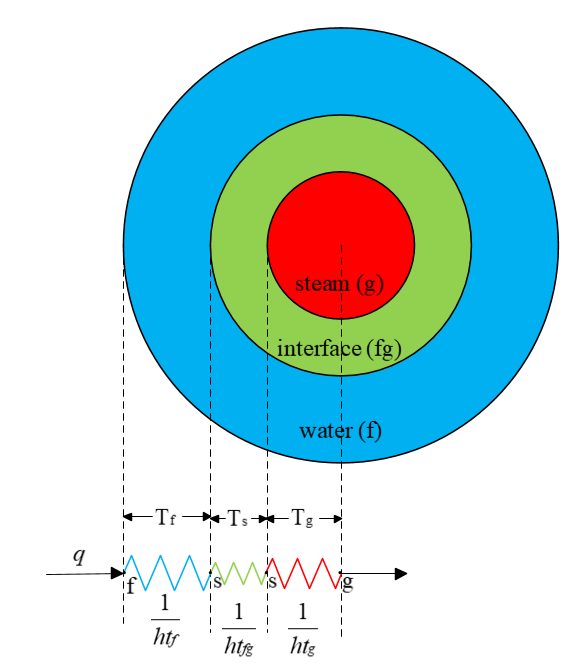
\includegraphics[height=5cm]{images/two resistance model.PNG}
    \caption{\centering Circuit diagram of a phasic volumes of steam and water and its interphase}
    \end{figure}
    \column{0.45\textwidth}
    \centering Interfacial Heat Transfer
    \begin{equation}\label{ihf_eqn}
    Q_g = -Q_f = ht_f{}_g A_f{}_g (T_f - T_g)
    \end{equation}
    \centering Interfacial Heat Transfer Coefficient
    \begin{equation}
    \frac{1}{ht_f{}_g} = \frac{1}{h_g} + \frac{1}{h_f}
    \end{equation}
    \begin{equation}
        ht_f{}_g = \frac{h_g h_f}{h_g + h_f}
    \end{equation}
\end{columns}
\end{frame}

\begin{frame}{Two-Resistance Model: Using Constants for Two-Resistors}
\begin{columns}
\column{0.45\textwidth}
Convective Heat Transfer Coefficient of Steam, $h_g$\cite{brucker1977direct,kosky2015exploring} 
\begin{align*}
    h_g = 10,000\:\frac{W}{m^{2}K}
\end{align*}
Convective Heat Transfer Coefficient of Water, $h_f$ \cite{kosky2015exploring,EngineeringToolbox}
\begin{align*}
    h_f = 1,000\:\frac{W}{m^{2}K}
\end{align*}
Free Convective Heat Transfer Coefficient of Air, $h_a$ \cite{kosky2015exploring}
\begin{align*}
    h_a = 25\:\frac{W}{m^{2}K}
\end{align*}
\column{0.45\textwidth}
Interfacial Heat Transfer Coefficient: 
\begin{itemize}
    \item Between Steam and Air
    \begin{align*}
        ht_g{}_a = \frac{10,000(25)}{10,000 + 25} = 24.938\frac{W}{m^{2}K}
    \end{align*}
    \item Between Water and Air
    \begin{align*}
        ht_w{}_a = \frac{1,000(25)}{1,000 + 25} = 24.390\frac{W}{m^{2}K}
    \end{align*}
    \item Between Steam and Water
    \begin{align*}
        ht_g{}_f = \frac{10,000(1,000)}{10,000 + 1,000} = 909.091\frac{W}{m^{2}K}
    \end{align*}
\end{itemize}
\end{columns}
\end{frame}

\begin{frame}{Interfacial Mass Transfer Between Steam and Water}
\begin{columns}
\column{0.45\textwidth}
\textbf{Thermal Phase Change Model:}
\begin{align*}
    \Dot{m_f{}_g} = \frac{ht_f A_f{}_g (T_s-T_f) + ht_g A_f{}_g (T_s - T_g)}{h_g{}_s - h_f{}_s}
    \end{align*}
    where:\\
    $h_{gs}$ and $h_{fs}$ are the phase enthalpies\\
    Note:\\
    Saturation Temperature ($T_{sat}$) is set to:
    \begin{align*}
        T_{sat} = 100^{\circ}C (373.15K)
    \end{align*}
\column{0.45\textwidth}
Condensation-Evaporation Model\cite{prakash1990two}\\
If $\Dot{m_f{}_g}\ge0$ (evaporation):
\begin{align*}
    h_f{}_s &= h_f(T_f)\\
    h_g{}_s &= h_g(T_{sat}) = 2,675.6 kJ/kg
\end{align*}
If $\Dot{m_f{}_g}<0$ (condensation):
\begin{align*}
    h_f{}_s &= h_f(T_{sat}) = 419.17 kJ/kg\\
    h_g{}_s &= h_g(T_{g})
\end{align*}
Latent Heat (L):
\begin{align*}
    L = h_{g}(T_{sat})-h_{f}(T_{sat}) = 2,256.43 kJ/kg
\end{align*}
\end{columns}
\end{frame}

\begin{frame}{Turbulence Model: Transport Equations for the Realizable \boldmath{$\kappa-\varepsilon$} model}\label{Rkvarepsilon_par}
    \begin{equation}\label{Rkappa_eqn}
    \frac{\partial}{\partial t} (\rho \kappa) + \frac{\partial}{\partial x_j}\big(\rho \kappa u_j\big) = \frac{\partial}{\partial x_j}\bigg[\Big(\mu + \frac{\mu_t}{\sigma_\kappa}\Big)\frac{\partial \kappa}{\partial x_j}\bigg] + G_\kappa + G_b -\rho\varepsilon-Y_M+S_\kappa
    \end{equation}
    \begin{equation}\label{Repsilon_eqn}
    \begin{split}
    \frac{\partial}{\partial}(\rho \varepsilon) 
    & + \frac{\partial}{\partial x_j}\big(\rho \varepsilon u_j\big) = \frac{\partial}{\partial x_j}\bigg[\Big(\mu + \frac{\mu_t}{\sigma_\varepsilon}\Big)\frac{\partial \varepsilon}{\partial x_j}\bigg]+ ... \\
    &... + \rho C_1 S_\varepsilon - \rho C_2 \frac{\varepsilon^2}{\kappa + \sqrt{\nu \varepsilon}} + C_1{}_\varepsilon \frac{\varepsilon}{\kappa} C_3{}_\varepsilon G_b + S_\varepsilon
    \end{split}
   \end{equation}
where,
\begin{equation}\label{C1_eqn}
    C_1 = max \bigg [0.43, \frac{\eta}{\eta + 5}\bigg], \eta = S\frac{\kappa}{\varepsilon}, S = \sqrt{2 S_i{}_j S_i{}_j}
\end{equation}
\end{frame}

\begin{frame}{Multiphase \boldmath{$\kappa-\varepsilon$} Turbulence Model for Each Phase}
    \begin{equation} \label{Rkappamulti_eqn}
    \begin{split}
    & \frac{\partial}{\partial t}\Big(\alpha_q\rho_q\kappa_q\Big) 
    + \nabla\cdot\Big(\alpha_q\rho_q \vec{U_q}\kappa_q\Big) = \\
    & \nabla\cdot\Bigg(\alpha_q\bigg(\mu_q + \frac{\mu_{t,q}}{\sigma_\kappa}\bigg)\nabla \kappa_q\Bigg) + \Big(\alpha_q G_{\kappa,q} - \alpha_q\rho_q\varepsilon_q\Big) +\dotsm \\
    &\dotsm + \sum_{p=1}^{N} K_{pq}\Big(C_{pq}\kappa_p - C_{qp}\kappa_q\Big) - \sum_{p=1}^{N} K_{pq} \Big(\vec{U_p}-\vec{U_q}\Big)\cdot\frac{\mu_{t,p}}{\alpha_p \sigma_p}\nabla \alpha_p +\dotsm \\
    &\dotsm + \sum_{p=1}^{N} K_{pq} \Big(\vec{U_p}-\vec{U_q}\Big)\cdot\frac{\mu_{t,q}}{\alpha_q \sigma_q}\nabla \alpha_q + \prod \kappa_q + \prod \kappa_p
    \end{split}
\end{equation}
\end{frame}

\begin{frame}{Multiphase \boldmath{$\kappa-\varepsilon$} Turbulence Model for Each Phase}
    \begin{equation}\label{Repsilonmulti_eqn}
    \begin{split}
      & \frac{\partial}{\partial t} \Big(\alpha_q\rho_q\varepsilon_q\Big) + \nabla\cdot\Big(\alpha_q\rho_q \vec{U_q}\varepsilon_q\Big) = \\ 
       & \nabla\cdot\Bigg(\alpha_q\bigg(\mu_q + \frac{\mu_{t,q}}{\sigma_\varepsilon}\bigg)\nabla \varepsilon_q\Bigg) + \alpha_q\rho_q C_{1\varepsilon} S_{k,q} \varepsilon_q - \alpha_q\rho_q C_{2\varepsilon} \frac{\varepsilon_q^2}{k_q + \sqrt{\nu_q \varepsilon_q}}+\dotsm \\
       &\dotsm + C_{3\varepsilon}\frac{\varepsilon_q}{\kappa_q}\bigg[\sum_{p=1}^{N} K_{pq}\Big(C_{pq}\kappa_p - C_{qp}\kappa_q\Big) - \sum_{p=1}^{N} K_{pq} \Big(\vec{U_p}-\vec{U_q}\Big)\cdot\frac{\mu_{t,p}}{\alpha_p \sigma_p}\nabla \alpha_p \\
      & + \sum_{p=1}^{N} K_{pq} \Big(\vec{U_p}-\vec{U_q}\Big)\cdot\frac{\mu_{t,q}}{\alpha_q \sigma_q}\nabla \alpha_q\bigg] + \prod \varepsilon_r
    \end{split}
\end{equation}
\end{frame}

\begin{frame}{Steam Equation of State\cite{ansys2011ansys}}
Steam Equation of State that relates the pressure (P) to the vapor density $\rho_{v}$ and the temperature (T) by a virial equation\cite{young1988equation},
    \begin{equation}
        P = \rho_{v}RT (1 + B\rho_{v} + C\rho_{v}^{2})
    \end{equation}
where B and C are the second and the third virial coefficients given the following empirical equations:
    \begin{equation}
        B = a_{1}(1 + \frac{\tau}{\alpha})^{-1} + a_{2}e^{\tau}(1 - e^{-\tau})^{\frac{5}{2}} + a_{3}\tau
    \end{equation}
where B is given in $\frac{m^{3}}{kg}$, $\tau=\frac{1500}{T}$, with T given in Kelvin (K)
\end{frame}

\begin{frame}{Steam Equation of State\cite{ansys2011ansys}}
        $\alpha = 10000.0, a_{1} = 0.0015, a_{2} = -0.000942, and a_{3} = -0.0004882$
    \begin{equation}
        C = a (\tau - \tau_{o})e^{-\alpha \tau} + b
    \end{equation}
where C is given in $\frac{m^{6}}{kg^{2}}$, $\tau = \frac{T}{647.286}$ with T given Kelvin, $\tau_{o}=0.8978$, $\alpha=11.16$, $a=1.772$ and $b=1.5e^{-06}$.\\
The two empirical functions that define the virial coefficients $B$ and $C$ cover the temperature range from 273 K to 1073 K.
\end{frame}

\begin{frame}{Steam Equation of State\cite{ansys2011ansys}}
    The vapor isobaric specific heat capacity $Cp_{v}$ is given by:
    \begin{equation}
       \begin{split}
           Cp_{v} = & Cp_{o}(T) 
                      \\ 
                    & + R[[(1-\alpha_{v}T)(B-B_{1})-B_{2}]\rho_{v}] \\
                    & + [(1-2\alpha_{v}T)C+\alpha_{v}TC_{1}-\frac{C_{2}}{2}]\rho_{v}^2] \\
       \end{split}
    \end{equation}
    where $Cp_{o}$ is in $\frac{kJ}{kg-K}$, and, \\
    $B_{1} = T \frac{dB}{dT}, C_{1} = T\frac{dC}{dT}, B_{2} = T^{2}\frac{dB^{2}}{dT^{2}}$, and $C_2 = T^{2} \frac{dC^{2}}{dT^{2}}$.
\end{frame}

\begin{frame}{Steam Equation of State\cite{ansys2011ansys}}
The vapor specific enthalpy, $h_{v}$ is given by:
    \begin{equation}
        h_{v} = h_{o}(T) + RT[(B - B_{1})\rho_{v} + (C-\frac{C_{1}}{2})\rho_{v}^2]
    \end{equation}
The vapor specific entropy, $s_{v}$ is given by:
    \begin{equation}
        s_{v} = s_{o}(T) + R[(B - B_{1})\rho_{v} + \frac{(C+{C_{1}})}{2}\rho_{v}^2]
    \end{equation}
\end{frame}

\begin{frame}{Steam Equation of State\cite{ansys2011ansys}}
    The isobaric specific heat at zero pressure is defined by the following empirical equation:
    \begin{equation}
        Cp_{o}(T) = \sum_{i=1}^{6} a_{i}T^{i-2}
    \end{equation}
    where $Cp_{o}$ is in $\frac{kJ}{kg-K}$, $a_{1}=46.0$,$a_{2}=1.47276$, $a_{3}=8.38930e-04$,$a_{4}=-2.19989e-07$, $a_{5}=2.46619e-10$, and $a_{6}=-9.70466e-14$.
\end{frame}

\begin{frame}{Steam Equation of State\cite{ansys2011ansys}}
    Both $h_{o}(T)$ and $s_{o}(T)$ are functions of temperature and they are defined by:
    \begin{equation}
        h_{o}(T) = \int Cp_{o} \,dT + h_{c}
    \end{equation}
    \begin{equation}
        s_{o}(T) = \int \frac{Cp_{o}}{T} \,dT + s_{c}
    \end{equation}
    where $h_{c}$ and $s_{c}$ are arbitrary constants.\\
    The vapor dynamic viscosity $\mu_{v}$ and thermal conductivity $k_{v}$ are also functions of temperature and were obtained from the journal entitled "The spontaneous condensation of steam in supersonic nozzles" by J.B. Young 1982\cite{young1982spontaneous}.
\end{frame}

\begin{frame}{T-s diagram showing the range of application of the equation of state\cite{young1988equation}}
    \begin{figure}
        \centering
        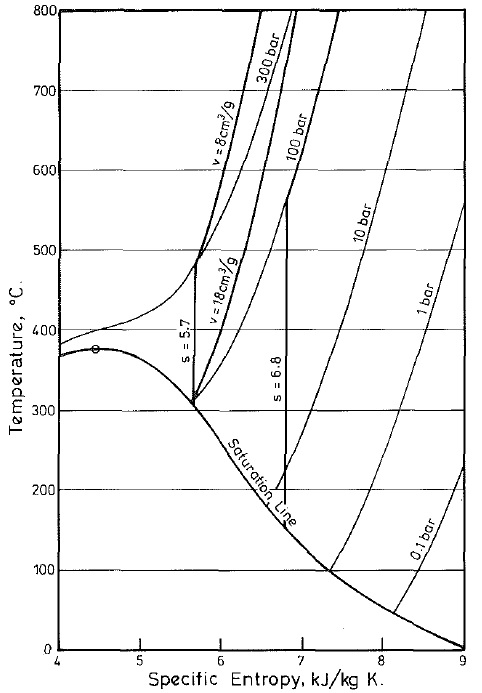
\includegraphics[height=5cm]{images/tsdiagramrangeofapplicationeos.jpg}
    \end{figure}
\end{frame}

\begin{frame}{Scalable Wall Functions\cite{ansys2017ansys}}
    The purpose of the scalable wall functions is to force the usage of the log law in conjunction with the standard wall functions approach. This is achieved by introducing a limiter in the y* calculations such that:
    \begin{equation}
        \tilde{y^*} = MAX(y^*, y_{limit}^*)
    \end{equation}
    where:\\
        $y_{limit}^* = 11.225.$\\
    The context of the scalable wall function is straightforward, thus, the \textbf{y* formulation used for any standard wall function is replaced by $\tilde{y^*}$.}
\end{frame}

\begin{frame}{Standard Wall Functions: Momentum Equation\cite{ansys2017ansys}}
\begin{columns}
  \column{0.45\textwidth}
    Law-of-the-wall for the dimensionless mean velocity yields:
  \begin{align*}
    U^* &= \frac{1}{\kappa}ln(Ey^*)\\
    U^* &\equiv U_p C_{\mu}^\frac{1}{4} k_p^\frac{1}{2} 
  \end{align*}
  The dimensionless distance from the wall expressed as:
  \begin{equation}
      y^* \equiv \frac{\rho C_{\mu}^\frac{1}{4} k_p^\frac{1}{2} y_p}{\mu}
  \end{equation}
  \scriptsize Note: Logarithmic law for the mean velocity is known to be valid for $30<y^*<300$, log-law is employed when $y^*>11.225$. When $y^*<11.225, U^*=y^*$.
  \column{0.45\textwidth}
  where:\\
  $\kappa = von\: Karmann\:constant\:(=0.4187)$ \\
  $E = empirical\:constant\:(9.793)$ \\
  $U_{p} = mean\:velocity\:of\:the\:fluid\:at\:the\:near-wall\:node\:P$ \\
  $k_p = turbulence\:kinetic\:energy\:at\:the\: near-wall\:node\:P$\\
  $y_p = distance\:from\:point\:P\:to\:the\:wall$\\
  $\mu = dynamic\:viscosity\:of\:the\:fluid$\\
  \scriptsize Note: In ANSYS Fluent, laws-of-the-wall for mean velocity and temperature are based on the wall unit,$y^*$, rather than $y^+ (\equiv \frac{\rho u_{\tau} y}{\mu})$. These quantities are approximately equal in equilibrium turbulent boundary layers.
\end{columns}
\end{frame}

\begin{frame}{Standard Wall Functions: Energy Equation\cite{ansys2017ansys}}
    \begin{equation*}
     T^* \equiv \frac{(T_w - T_p)\rho C_p k_p^\frac{1}{2}}{\Dot{q}} = \left\{
        \begin{array}{ll}
            Pry^* + \frac{1}{2} \rho Pr \frac{C_\mu^\frac{1}{4}k_p^\frac{1}{2}}{\Dot{q}} U_p^2 & \quad y^* < y_T^* \\
            Pr_t[\frac{1}{\kappa}ln(Ey^*)+\rho]+\cdots \\
            \cdots + \frac{1}{2} \rho Pr \frac{C_\mu^\frac{1}{4}k_p^\frac{1}{2}}{\Dot{q}}[Pr_tU_p^2 + (Pr-Pr_t)U_c^2]  & \quad y^* > y_T^* 
        \end{array}
    \right.
    \end{equation*}
  where P is computed as:
    \begin{equation}
        P = 9.24 \bigg[\bigg(\frac{Pr}{Pr_t}\bigg)^\frac{3}{4}-1\bigg]\bigg[1 + 0.28e^\frac{-0.007Pr}{Pr_t}\bigg]
    \end{equation}
    \label{stdwallfuncenergyeqn}
\end{frame}

\begin{frame}{Standard Wall Functions: Energy Equation}
    In slide \ref{stdwallfuncenergyeqn}:\\
    $k_p = turbulent\:kinetic\:energy\:at\:the\:first near-wall\:node\:P$\\
    $\rho = density\:of\:the\:fluid$\\
    $C_p = specific\:heat\:of\:fluid$\\
    $\Dot{q}= wall\:heat\: flux$\\
    $T_p = temperature\:at\:the\:first\:near-wall\:node\:P$\\
    $T_w = temperature\:at\:the\:wall$\\
    $Pr = molecular\:Prandtl\:number\:(\mu C_p/k_f)$\\
    $Pr_t = turbulent\:Prandtl\:number(0.85\:at\:the\:wall)$\\
    $U_c = mean\:velocity\:magnitude\:at\:y^*=y_T^*$
\end{frame}

\begin{frame}{Heat Transfer Coefficient for $CO_2$: Hughmark Model}
    \begin{equation*}
     Nu_p  = \left\{
        \begin{array}{lll}
            2 + 0.6 Re_p^\frac{1}{2} Pr^\frac{1}{3} & \quad 0\leq Re_p < 776.06 & \quad 0\leq Pr < 250 \\
            2 + 0.27 Re_p^{0.62} Pr^\frac{1}{3}  & \quad 776.06\leq Re_p  & \quad 0\leq Pr < 250
        \end{array}
    \right.
    \end{equation*}
    \begin{equation*}
        h_p = \frac{k_p Nu_p}{d_g}
    \end{equation*}
    where:\\
    $Nu_p = Nusselt\:number\:of\:the\:p^{th}\:phase$\\
    $Re = Reynolds\:number\:of\:the\:p^{th}\:phase$\\
    $Pr = Prandtl\:number$\\
    $h_p = heat\:transfer\:coefficient\:of\:the\:p^{th}\:phase,$\\
    $k_p = thermal\:conductivity\:of\:the\:p^{th}\:phase, d_g = particle\:diameter$
\end{frame}